%%% Local Variables:
%%% mode: latex
%%% TeX-master: t
%%% End:

\chapter{引言}
\label{cha:intro}

\section{粒子物理} 
粒子物理(又称高能物理)是一门研究构成物质的基本组成粒子和它们之间基本相互作用的一门学科。对粒子物理的探讨最早可以追溯到公元前四世纪的原子论,古希腊哲学家德谟克利特(Democritus)认为世间万物均是由原子(atom)所构成,它是一种肉眼不可见的、永远处于运动中的不可分割的微观粒子,任何物质含有的这种微观粒子越多,它的质量就会越大。

直到19世纪末20世纪初,人类才真正开始通过实验手段对粒子物理进行研究。1892年,英国物理学家约瑟夫汤姆逊(J. J. Thomson)通过实验证实阴极射线是由一种基本粒子所构成~\cite{electron},这种粒子在不同材料发射出来的阴极射线中都具有相同的电荷质量比值,随后这种粒子就被命名为电子。1911年,卢瑟福(Ernest Rutherford)通过实验发现$\alpha$粒子撞击金箔后会发生大角度散射,由此提出了原子的核式结构模型并发现了中子。1919年,卢瑟福又通过$\alpha$粒子轰击靶原子发现了质子~\cite{proton}。至此,原子的经典核式结构被完整构建出来:原子是由外围带负电的电子和中心带正电的原子核所构成,原子核由不带电的中子和带正电的质子所构成。这一结构让人类首次对微观世界的基本粒子有了一个清晰的物理图像,构成了近代粒子物理的基础。

与此同时,漂浮在物理学上空的“两朵乌云”:黑体辐射~\cite{blackbody}和迈克尔逊-莫雷干涉实验~\cite{shankland1964michelson}也为人类带来了量子力学和狭义相对论,正是这两项发现构成了现代粒子物理学的基础。1900年,普朗克(Max Planck)在对黑体辐射的解释中首次引入了量子化的概念~\cite{Gearhart2009},认为电磁场只能以量子化的形式发射和吸收电磁波。1905年,爱因斯坦(Albert Einstein)利用光量子的概念对光电效应成功地进行了理论解释~\cite{einstein1905heuristic}。1913年,玻尔(Niels Bohr)提出了氢原子的量子化轨道模型~\cite{bohr1913constitution},成功解释了氢原子光谱数据。1923年,德布罗意(Louis de Broglie)提出了波粒二象性原理~\cite{waveparticle,menzel1960fundamental,greene2000elegant},认为任何基本粒子都具有波动性。在此基础上,海森堡(Heisenberg)于1925年提出不确定性原理~\cite{uncer1,uncer2,uncer3},认为我们无法同时精确测量粒子的位置和动量。薛定谔(Schrödinger)也于次年提出了薛定谔方程~\cite{schrodinger1,schrodinger2},用于描述波函数的量子行为。随后玻恩提出了概率幅的概念,成功地解释了波函数的物理意义。然而,薛定谔的波函数方程并不具备洛伦兹不变性,而后者正是狭义相对论的基本假设之一,这就意味着薛定谔方程只能描述基本粒子的非相对论性部分。真正将量子力学和狭义相对论统一起来的是英国理论物理学家狄拉克(Paul Dirac)。狄拉克方程描述了所有自旋为$\frac{1}{2}$的质量不为0的基本粒子的量子力学行为,它完美地解释了氢原子光谱的精细结构,并且预言了反粒子的存在。狄拉克认为波函数一共有四个部分,包含两个自旋为$\frac{1}{2}$的粒子,每个粒子包含两部分:一部分用于描述粒子;另一部分用于描述反粒子。1932年,正电子被安德森(Carl David Anderson)所发现,证实了狄拉克方程的正确性。至此,由于微观粒子的运动可以通过波动方程来描述,“场”的概念逐渐被人们重视起来。随后,在费曼(Feynman)、朝永振一郎(Tomonaga)以及施温格(Schwinger)等人的工作下,量子电动力学(QED)被构建出来,人们认识到电磁相互作用是通过电磁场交换光子得到的。1954年,杨振宁和米尔斯(Robert Mills)创建了非阿贝尔规范理论~\cite{PhysRev.96.191}(Yang–Mills 理论),开始从对称性的角度来理解粒子之间的相互作用。谢尔登·格拉肖(Sheldon Glashow)、温伯格(Steven Weinberg)和阿卜杜勒·萨拉姆(Abdus Salam)也于1960年基于Yang–Mills理论统一了电磁相互作用和通过贝塔衰变实验发现的弱相互作用,创建了电弱统一理论。而对于描述原子核内部的相互作用力,Yukawa在1930年曾提出可以用一种全新的强相互作用力来描述,这种作用力可以通过交换$\pi$介子来实现。1964年,弗朗索瓦·恩格勒(François Englert)和彼得·希格斯(Peter Higgs)提出对称性自发破缺机制~\cite{PhysRevLett.13.321, brout1998spontaneous, PhysRevLett.13.508},预言了希格斯玻色子的存在。1971年,哈拉尔德·弗里奇(Harald Fritzsch)、默里·盖尔曼(Murray Gell-Mann)和海因里希·洛伊特维勒(Heinrich Leutwyler)发现强相互作用力也可以通过非阿贝尔规范理论来描述,他们在此基础上建立了量子色动力学(QCD)并提出了“色荷”的概念,认为质子和中子是由三个夸克所构成,每种夸克都有三种颜色。2012年,希格斯粒子(Higgs)在欧洲核子研究中心(CERN)被发现~\cite{HiggsdiscoveryAtlas, Chatrchyan:2012ufa, Chatrchyan:2013lba},标准模型的最后一块拼图被找到。

至此,现代粒子物理学基础标准模型(the Standard Model, SM)正式建立,这个理论囊括了描述电磁相互作用和弱相互作用的电弱统一理论以及描述强相互作用的量子色动力学,但是却无法描述仅剩的万有引力作用力。标准模型的建立让人们对组成物质的基本粒子以及它们之间的相互作用有了深刻的了解,它成功解释了一些粒子物理学上观测到的实验现象,但仍然存在一些目前标准模型无法解释的物理现象,比如:暗物质、暗能量、中微子质量等等。这就意味着标准模型并不是一个完美地理论,我们仍然需要寻找超出标准模型的新物理(Beyond Standard Model, BSM)。

\section{标准模型}

粒子物理标准模型描述了目前人类所了解到的所有微观粒子的基本运动以及粒子之间的基本相互作用。到目前为止,人类一共发现并认识了17种微观粒子,如图~\ref{fig:c01f01}。根据对微观世界的基本理解,这些基本粒子可以大致划分为构成物质的夸克和轻子、传递相互作用的规范玻色子以及通过对称性自发破缺机制使得所有基本粒子获得质量的希格斯粒子。每种粒子都有各自对应的内禀属性,比如:电荷、自旋和色荷。

\begin{figure}[!htbp]
    \centering
    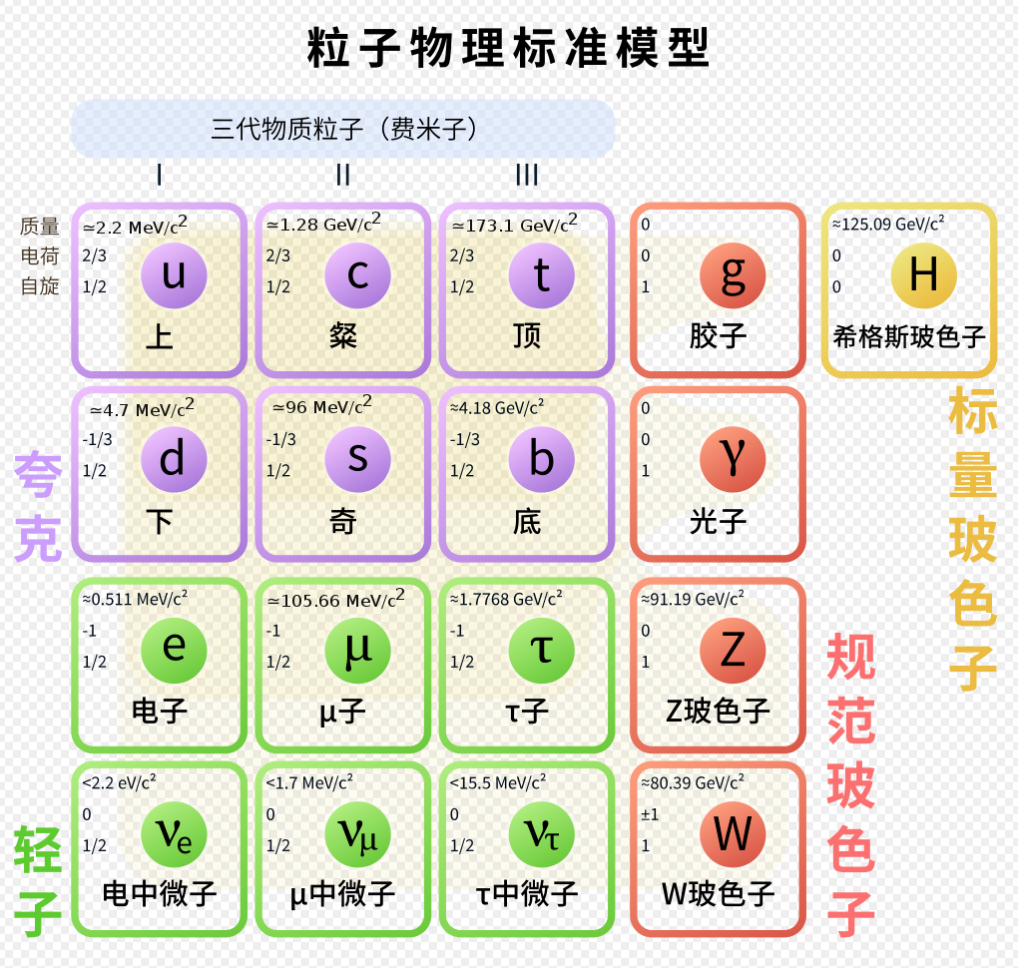
\includegraphics[width=0.50\textwidth]{figures/chapter01/SM.jpg}
    \bicaption{\quad \centering 粒子物理标准模型示意图~\cite{particlephys}}{\quad \centering Schematic diagram of Standard Model of particle physics~\cite{particlephys}}
    \label{fig:c01f01}
\end{figure}

其中,电荷用以描述微观粒子的带电荷量,根据不同微观粒子的带电性质,可以分为带正电荷的粒子、带负电荷的粒子以及不带电的中性粒子。在标准模型中,夸克、轻子和W玻色子带有电荷,剩下的中微子、胶子、光子以及希格斯粒子不带电,任何带电粒子都有与之对应的带相反电荷的反粒子。

自旋用以描述基本粒子的转动角动量这一性质,它的值是量子化的并且无法被改变。按照基本粒子的自旋特性,可以将基本粒子分为自旋为整数的玻色子和自旋为半整数的费米子。玻色子遵从玻色-爱因斯坦统计,对于全同的玻色子,波函数具有对称性,交换其中的两个粒子并不会改变波函数,这类粒子可以具有相同的量子态;而费米子遵从费米-狄拉克统计,对于全同的费米子,波函数具有反对称性,交换其中的两个粒子会使得波函数增加一个负号,这类粒子遵守泡利不相容原理,两个全同的费米子不能占据同样的量子态。在标准模型中,规范玻色子和希格斯粒子属于玻色子,夸克和轻子属于费米子。

色荷是夸克和胶子的一种内禀属性,用于描述处于不同状态的夸克和胶子。对于夸克来说,每种夸克有三种颜色:红色、绿色和蓝色,夸克的色荷可以处于这三种颜色之间;而胶子的色荷是由两种颜色混合而成,在量子色动力学中一共存在8种胶子。由于在量子色动力学中“色禁闭”效应的存在,由多个正反夸克构成的强子具有色中性的性质;而胶子的渐进自由特性使得它能够作为传递强相互作用的基本粒子。

基本粒子之间的相互作用可以根据相互作用的强度分为弱相互作用、电磁相互作用以及强相互作用,传递相互作用的媒介粒子分别为W、Z玻色子、光子以及胶子,对这些相互作用的描述可以通过规范场论来实现。

\subsection{电弱统一理论}

对于弱相互作用和电磁相互作用,电弱统一理论对其进行了成功地解释。电弱对称性发生自发破缺后的拉氏量可以表示为下面的形式:
\begin{equation}\label{eq:1-1}
    \mathcal{L}_{\mathrm{EW}}=\mathcal{L}_{\mathrm{K}}+\mathcal{L}_{\mathrm{N}}+\mathcal{L}_{\mathrm{C}}+\mathcal{L}_{\mathrm{H}}+\mathcal{L}_{\mathrm{HV}}+\mathcal{L}_{\mathrm{WWV}}+\mathcal{L}_{\mathrm{WWVV}}+\mathcal{L}_{\mathrm{Y}}
\end{equation}

动力学项$\mathcal{L}_{\mathrm{K}}$给出了拉氏量中的所有二次项(方程~\eqref{eq:1-2}),其中包含了费米子、规范玻色子、希格斯粒子的动力学项和质量项,$A_{\mu\nu}$、$Z_{\mu,\nu}$、$W^{\pm}_{\mu\nu}$分别表示对应的规范场,$f$表示费米子场,$H$表示希格斯场;中性流$\mathcal{L}_{\mathrm{N}}$(方程~\eqref{eq:1-3})和带电流$\mathcal{L}_{\mathrm{C}}$(方程~\eqref{eq:1-4})部分包含了费米子和规范玻色子之间的相互作用,其中CKM矩阵$M_{i j}^{\mathrm{CKM}}$确定了夸克的质量本征态和弱相互作用本征态之间的混合角度,$J_{\mu}^{em}$表示电磁流,$J_{\mu}^{3}$表示中性弱流;$\mathcal{L}_{\mathrm{H}}$描述了希格斯粒子的三顶点、四顶点自耦合相互作用项(方程~\eqref{eq:1-5});$\mathcal{L}_{\mathrm{HV}}$描述了希格斯粒子和规范矢量玻色子之间的相互作用(方程~\eqref{eq:1-6});$\mathcal{L}_{\mathrm{WWV}}$(方程~\eqref{eq:1-7})和$\mathcal{L}_{\mathrm{WWVV}}$(方程~\eqref{eq:1-8})描述了规范玻色子的三顶点、四顶点自耦合相互作用;$\mathcal{L}_{\mathrm{Y}}$描述了费米子和希格斯场之间的Yukawa相互作用(方程~\eqref{eq:1-9})。
\begin{equation}\label{eq:1-2}
    \begin{array}{r}
        \mathcal{L}_{\mathrm{K}}=\sum_{f} \bar{f}(i \not\partial -m_{f}) f-\frac{1}{4} A_{\mu \nu} A^{\mu \nu}-\frac{1}{2} W_{\mu \nu}^{+} W^{-\mu \nu}+m_{W}^{2} W_{\mu}^{+} W^{-\mu} \\
        -\frac{1}{4} Z_{\mu \nu} Z^{\mu \nu}+\frac{1}{2} m_{Z}^{2} Z_{\mu} Z^{\mu}+\frac{1}{2}(\partial^{\mu} H)(\partial_{\mu} H)-\frac{1}{2} m_{H}^{2} H^{2}
    \end{array}
\end{equation}

\begin{equation}\label{eq:1-3}
    \mathcal{L}_{\mathrm{N}}=e J_{\mu}^{\mathrm{em}} A^{\mu}+\frac{g}{\cos \theta_{W}}\left(J_{\mu}^{3}-\sin ^{2} \theta_{W} J_{\mu}^{\mathrm{em}}\right) Z^{\mu}
\end{equation}

\begin{equation}\label{eq:1-4}
    \mathcal{L}_{\mathrm{C}}=-\frac{g}{\sqrt{2}}\left[\bar{u}_{i} \gamma^{\mu} \frac{1-\gamma^{5}}{2} M_{i j}^{\mathrm{CKM}} d_{j}+\bar{\nu}_{i} \gamma^{\mu} \frac{1-\gamma^{5}}{2} e_{i}\right] W_{\mu}^{+}+\text {h.c. }
\end{equation}

\begin{equation}\label{eq:1-5}
    \mathcal{L}_{\mathrm{H}}=-\frac{g m_{\mathrm{H}}^{2}}{4 m_{\mathrm{W}}} H^{3}-\frac{g^{2} m_{\mathrm{H}}^{2}}{32 m_{\mathrm{W}}^{2}} H^{4}
\end{equation}

\begin{equation}\label{eq:1-6}
    \mathcal{L}_{\mathrm{HV}}=\left(g m_{\mathrm{HV}}+\frac{g^{2}}{4} H^{2}\right)\left(W_{\mu}^{+} W^{-\mu}+\frac{1}{2 \cos ^{2} \theta_{\mathrm{W}}} Z_{\mu} Z^{\mu}\right)
\end{equation}

\begin{equation}\label{eq:1-7}
    \begin{aligned}
        \mathcal{L}_{\mathrm{WWV}} & =-i g[\left(W_{\mu \nu}^{+} W^{-\mu}-W^{+\mu} W_{\mu \nu}^{-}\right)\left(A^{\nu} \sin \theta_{\mathrm{W}}-Z^{\nu} \cos \theta_{\mathrm{W}}\right) \\
        &+W_{\nu}^{-} W_{\mu}^{+}\left(A^{\mu \nu} \sin \theta_{\mathrm{W}}-Z^{\mu \nu} \cos \theta_{\mathrm{W}}\right)]
    \end{aligned}
\end{equation}

\begin{equation}\label{eq:1-8}
    \begin{aligned}
    & \mathcal{L}_{\mathrm{WWVV}} =-\frac{g^{2}}{4}\{ {\left[2 W_{\mu}^{+} W^{-\mu}+\left(A_{\mu} \sin \theta_{\mathrm{W}}-Z_{\mu} \cos \theta_{\mathrm{W}}\right)^{2}\right]^{2} } \\
    & \left.-\left[W_{\mu}^{+} W_{\nu}^{-}+W_{\nu}^{+} W_{\mu}^{-}+\left(A_{\mu} \sin \theta_{\mathrm{W}}-Z_{\mu} \cos \theta_{\mathrm{W}}\right)(A_{\nu} \sin \theta_{\mathrm{W}}-Z_{\nu} \cos \theta_{\mathrm{W}}\right)\right]^{2} \}
\end{aligned}
\end{equation}

\begin{equation}\label{eq:1-9}
    \mathcal{L}_{\mathrm{Y}}=-\sum_{f} \frac{g m_{f}}{2 m_{\mathrm{W}}} \bar{f} f H
\end{equation}

\subsection{量子色动力学}

对于夸克和胶子之间的强相互作用力,量子色动力学对其进行了阐述。规范不变的量子色动力学拉氏量可以写为如下形式:
\begin{equation}\label{eq:1-10}
    \mathcal{L}_{\mathrm{QCD}}=\bar{\psi}_{i}\left(i \gamma^{\mu}\left(D_{\mu}\right)_{i j}-m \delta_{i j}\right) \psi_{j}-\frac{1}{4} G_{\mu \nu}^{a} G_{a}^{\mu \nu}
\end{equation}

其中,$\psi_{i}(x)$是夸克场,它是时空的函数;$G_{\mu \nu}^{a}$表示规范不变的胶子场强张量,具体表达式为(方程~\eqref{eq:1-11}),$\mathcal{A}_{\mu}^{a}(x)$表示胶子场;变量$m$和$g$分别对应于夸克的质量和耦合顶点参数。
\begin{equation}\label{eq:1-11}
    G_{\mu \nu}^{a}=\partial_{\mu} \mathcal{A}_{\nu}^{a}-\partial_{\nu} \mathcal{A}_{\mu}^{a}+g f^{a b c} \mathcal{A}_{\mu}^{b} \mathcal{A}_{\nu}^{c}
\end{equation}

\subsection{超出标准模型的新物理}

标准模型可以解释目前粒子物理实验上观测到的绝大多数的物理现象。然而,标准模型并不是一个完美地理论,仍然存在许多标准模型无法解释的物理现象,比如说:暗物质、暗能量、中微子质量、正反物质不对称等等。这就意味着我们仍然需要寻找超出标准模型的新物理。

根据当前宇宙学标准模型的计算,宇宙中大约 27\% 是暗物质;68\% 是暗能
量。构成恒星、行星和生物的介子只占宇宙总质量的大约 5\%。这也就是说,标准模型只能解释宇宙中的极少部分组成。到目前为止,人们认为暗物质的可能的存在形式是粒子形式,对应的可能粒子主要有以下几种:
\begin{itemize}
    \item 低质量玻色子:包括量子色动力学轴子~\cite{Bandyopadhyay_2019}、类轴子和模糊冷暗物质~\cite{PhysRevLett.85.1158}等;
    \item 中微子:包括标准模型中微子和惰性中微子~\cite{Boyarsky_2019};
    \item 弱尺度下的新粒子:比如超对称~\cite{1966PThPh..36.1266M}、额外维度~\cite{rizzo2004pedagogical}、有效场论~\cite{Criado_2021}等等;
    \item 其他粒子:比如大质量弱相互作用粒子~\cite{Jungman_1996}(Weakly Interacting Massive Particles,WIMPs)、自相互作用的暗物质~\cite{PhysRevLett.84.3760}等等。
\end{itemize}

在标准模型中,希格斯玻色子作为唯一的标量粒子,赋予了所有基本粒子以质量,这就使得暗物质粒子的质量起源可能和希格斯粒子有关。因此,寻找希格斯粒子与暗物质粒子的相互作用是一个前沿热点课题。近年来,LHC上的ATLAS实验和CMS实验都对以上可能的暗物质粒子进行了寻找,对许多新物理模型给出了排除限制。当然,其中也不乏利用希格斯粒子来对暗物质进行寻找。其中,对希格斯粒子衰变到不可探测粒子的测量就是一个很好的例子。在标准模型中,由于中微子不具有质量并且几乎不与任何物质发生相互作用,使得中微子成为了在对撞机中唯一不能够被探测到的粒子。根据标准模型的计算,希格斯粒子衰变到中微子的分支比仅占0.1\%~\cite{Dittmaier:2011ti}。而根据CMS实验的最新测量结果,希格斯粒子衰变到不可探测粒子的分支比排除上限仅为18\%~\cite{Hinv}。这就意味着它们中间可能会包含有无法被探测器捕捉到的超出标准模型的新粒子的存在,比如长寿命的暗物质粒子,使得测量结果远超出标准模型的计算。因此,寻找这类超出标准模型的新物理具有非常重要的物理意义。

\section{类轴子}
\label{sec:first}
类轴子(Axion-Like Particles, ALPs)模型描述了一种全新的基本粒子,这种粒子是一个规范单态的赝标量粒子,并且具有近似的平移对称性这一特性,因此它的质量通常会比电弱标度甚至QCD标度更小。对于类轴子的描述可以通过有效场论来完成~\cite{PhysRevLett.119.031802,Bauer:2017ris},最简单的维度小于5的有效拉氏量可以写为:
\begin{equation}\label{eq:1-12}
    \begin{aligned}
    \mathcal{L}_{\text {eff }}^{D \leq 5}= & \frac{1}{2}(\partial_{\mu} a)\left(\partial^{\mu} a\right)-\frac{m_{a, 0}^{2}}{2} a^{2}+\frac{\partial^{\mu} a}{\Lambda} \sum_{F} \bar{\psi}_{F} \boldsymbol{C}_{F} \gamma_{\mu} \psi_{F} \\
    & +g_{s}^{2} C_{G G} \frac{a}{\Lambda} G_{\mu \nu}^{A} \tilde{G}^{\mu \nu, A}+g^{2} C_{W W} \frac{a}{\Lambda} W_{\mu \nu}^{A} \tilde{W}^{\mu \nu, A}+g^{\prime 2} C_{B B} \frac{a}{\Lambda} B_{\mu \nu} \tilde{B}^{\mu \nu},
    \end{aligned}
\end{equation}
其中包含了不满足平移对称性的质量项$m_{a, 0}^{2}$;$G_{\mu \nu}^{A}$、$W_{\mu \nu}^{A}$和$B_{\mu \nu}$分别表示了$SU(3)_c$、$SU(2)_L$和$U(1)_Y$场强张量,$g_s$、$g$和$g'$分别表示了对应的耦合常数;$\Lambda$表示新物理的标度,这是全局对称性破缺的特征尺度。

然而在树图水平上,五阶算符不存在$H\rightarrow Z\gamma$的耦合顶点,这一衰变道被圈图效应所压低,使得在探测器上对这一衰变道的寻找变得极为困难。但是,我们可以通过构建更高阶的算符来产生树图阶的贡献。六维以上的有效拉氏量可以写为:
\begin{equation}\label{eq:1-13}
    \mathcal{L}_{\mathrm{eff}}^{D \geq 6}=\frac{C_{a h}}{\Lambda^{2}}(\partial_{\mu} a)\left(\partial^{\mu} a\right) \phi^{\dagger} \phi+\frac{C_{a h}^{\prime}}{\Lambda^{2}} m_{a, 0}^{2} a^{2} \phi^{\dagger} \phi+\frac{C_{Z h}^{(7)}}{\Lambda^{3}}\left(\partial^{\mu} a\right)\left(\phi^{\dagger} i D_{\mu} \phi+\text { h.c. }\right) \phi^{\dagger} \phi+\ldots 
\end{equation}
其中前两项给出了对$H\rightarrow aa$衰变道的贡献;第三项给出了领头阶的$H\rightarrow Z\gamma$树图衰变贡献。在经过电弱对称性破缺后,有效拉氏量~\eqref{eq:1-12}给出了类轴子和$\gamma\gamma$、$\gamma Z$以及$ZZ$之间的耦合参数,对应的表达式可以写为:

\begin{equation}\label{eq:1-14}
    \mathcal{L}_{\text {eff }}^{D \leq 5} \ni e^{2} C_{\gamma \gamma} \frac{a}{\Lambda} F_{\mu \nu} \tilde{F}^{\mu \nu}+\frac{2 e^{2}}{s_{w} c_{w}} C_{\gamma Z} \frac{a}{\Lambda} F_{\mu \nu} \tilde{Z}^{\mu \nu}+\frac{e^{2}}{s_{w}^{2} c_{w}^{2}} C_{Z Z} \frac{a}{\Lambda} Z_{\mu \nu} \tilde{Z}^{\mu \nu}
\end{equation}

至此,类轴子模型的有效拉氏量基本构建完成。拉氏量~\eqref{eq:1-12}给出了类轴子衰变到一对标准模型规范玻色子和费米子的耦合参数,比如:$a\rightarrow \gamma\gamma$、$a\rightarrow \ell\ell$、$a\rightarrow q\bar{q}$和$a\rightarrow gg$。对于类轴子的产生模式,拉氏量~\eqref{eq:1-13}和~\eqref{eq:1-14}分别给出了$H\rightarrow aa$和$H\rightarrow Za$的一阶圈图修正和领头阶树图的贡献。

\subsection{缪子反常磁矩}

自旋磁矩作为基本粒子的内禀属性之一,通常表述为g因子,可以通过实验或者理论计算得到。根据狄拉克方程预言,电子或者缪子的g因子为2,这对应于量子电动力学中的树图解释。然而,高阶圈图修正会对g因子的计算产生影响。此时,我们将实验观测结果和树图结果的差值百分比定义为反常磁矩$a$:
\begin{equation}\label{eq:1-15}
    a = \frac{g-2}{2}
\end{equation}
反常磁矩的测量结果和理论计算结果对精确检验量子电动力学的正确性具有非常重要的意义。目前,根据Muon g-2合作组的最新测量,缪子反常磁矩的测量结果为$a=0.00116592061(41)$\cite{abi2021measurement}。然而,在考虑了电弱修正和强子修正之后,理论计算和实验结果之间的偏差仍然达到了4.2个标准偏差,这就意味着其间很有可能存在超出标准模型的新物理。

\begin{figure}[!htbp]
    \centering
    %trim option's parameter order: left bottom right top
    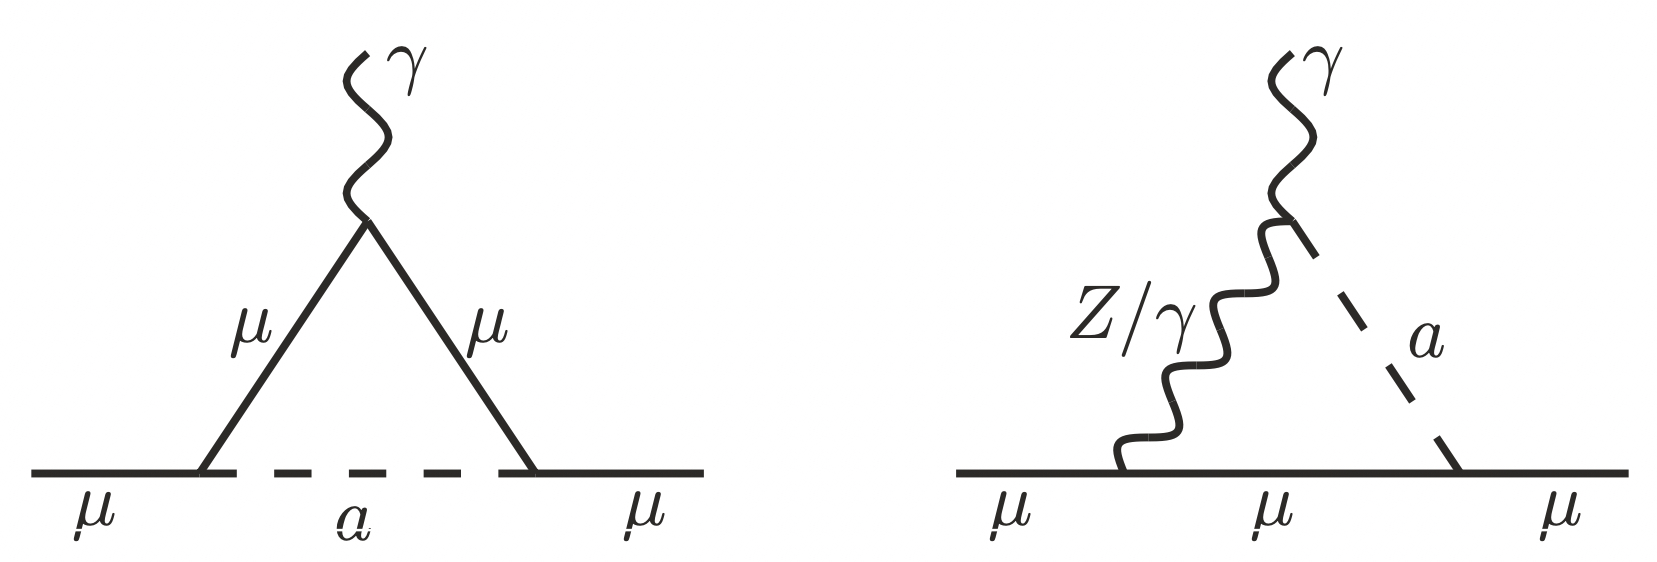
\includegraphics[width=0.60\textwidth]{figures/chapter01/ALP_g_2.jpg}
    \bicaption{\quad \centering 类轴子模型单圈费曼图对缪子反常磁矩的贡献~\cite{Bauer:2017ris}}{\quad \centering One-loop Feyman diagrams contributing to the anomalous magnetic moment of the muon for Axion-Like Particles Model~\cite{Bauer:2017ris}}
    \label{fig:c01f02}
\end{figure}

类轴子模型可以为缪子反常磁矩的偏差提供理论解释。在单圈图阶段,类轴子模型有效拉氏量对缪子反常磁矩的贡献可以通过费曼图\ref{fig:c01f02}进行描述。通过计算,类轴子模型引起的新物理贡献可以表示为:
\begin{equation}\label{eq:1-16}
    \begin{array}{c}
    \delta a_{\mu}=\frac{m_{\mu}^{2}}{\Lambda^{2}}\left\{K_{a_{\mu}}(\mu)-\frac{\left(c_{\mu \mu}\right)^{2}}{16 \pi^{2}} h_{1}\left(\frac{m_{a}^{2}}{m_{\mu}^{2}}\right)-\frac{2 \alpha}{\pi} c_{\mu \mu} C_{\gamma \gamma}\left[\ln \frac{\mu^{2}}{m_{\mu}^{2}}+\delta_{2}+3-h_{2}\left(\frac{m_{a}^{2}}{m_{\mu}^{2}}\right)\right]\right. \\
    \left.-\frac{\alpha}{2 \pi} \frac{1-4 s_{w}^{2}}{s_{w} c_{w}} c_{\mu \mu} C_{\gamma Z}\left(\ln \frac{\mu^{2}}{m_{Z}^{2}}+\delta_{2}+\frac{3}{2}\right)\right\} 
    \end{array}
\end{equation}
其中,
\begin{equation}\label{eq:1-17}
    \begin{array}{l}
    h_{1}(x)=1+2 x+x(1-x) \ln x-2 x(3-x) \sqrt{\frac{x}{4-x}} \arccos \frac{\sqrt{x}}{2} \\
    h_{2}(x)=1-\frac{x}{3}+\frac{x^{2}}{6} \ln x+\frac{2+x}{3} \sqrt{x(4-x)} \arccos \frac{\sqrt{x}}{2}
    \end{array}
\end{equation}

图\ref{fig:c01f03}展示了可以用来解释实验上所观测到的缪子反常磁矩的类轴子模型的参数空间。其中,红色、橘色和黄色范围分别表示可以在68\%、95\%和99\%的置信度上解释实验上观测到的缪子反常磁矩的类轴子模型的参数空间范围;灰色区域表示可以被BaBar实验中对暗光子的寻找所排除的参数空间范围。目前为止,仍然没有实验结果可以完全排除类轴子模型对缪子反常磁矩的贡献。因此,类轴子的寻找对了解缪子反常磁矩具有非常重要的物理意义。

\begin{figure}[!htbp]
    \centering
    %trim option's parameter order: left bottom right top
    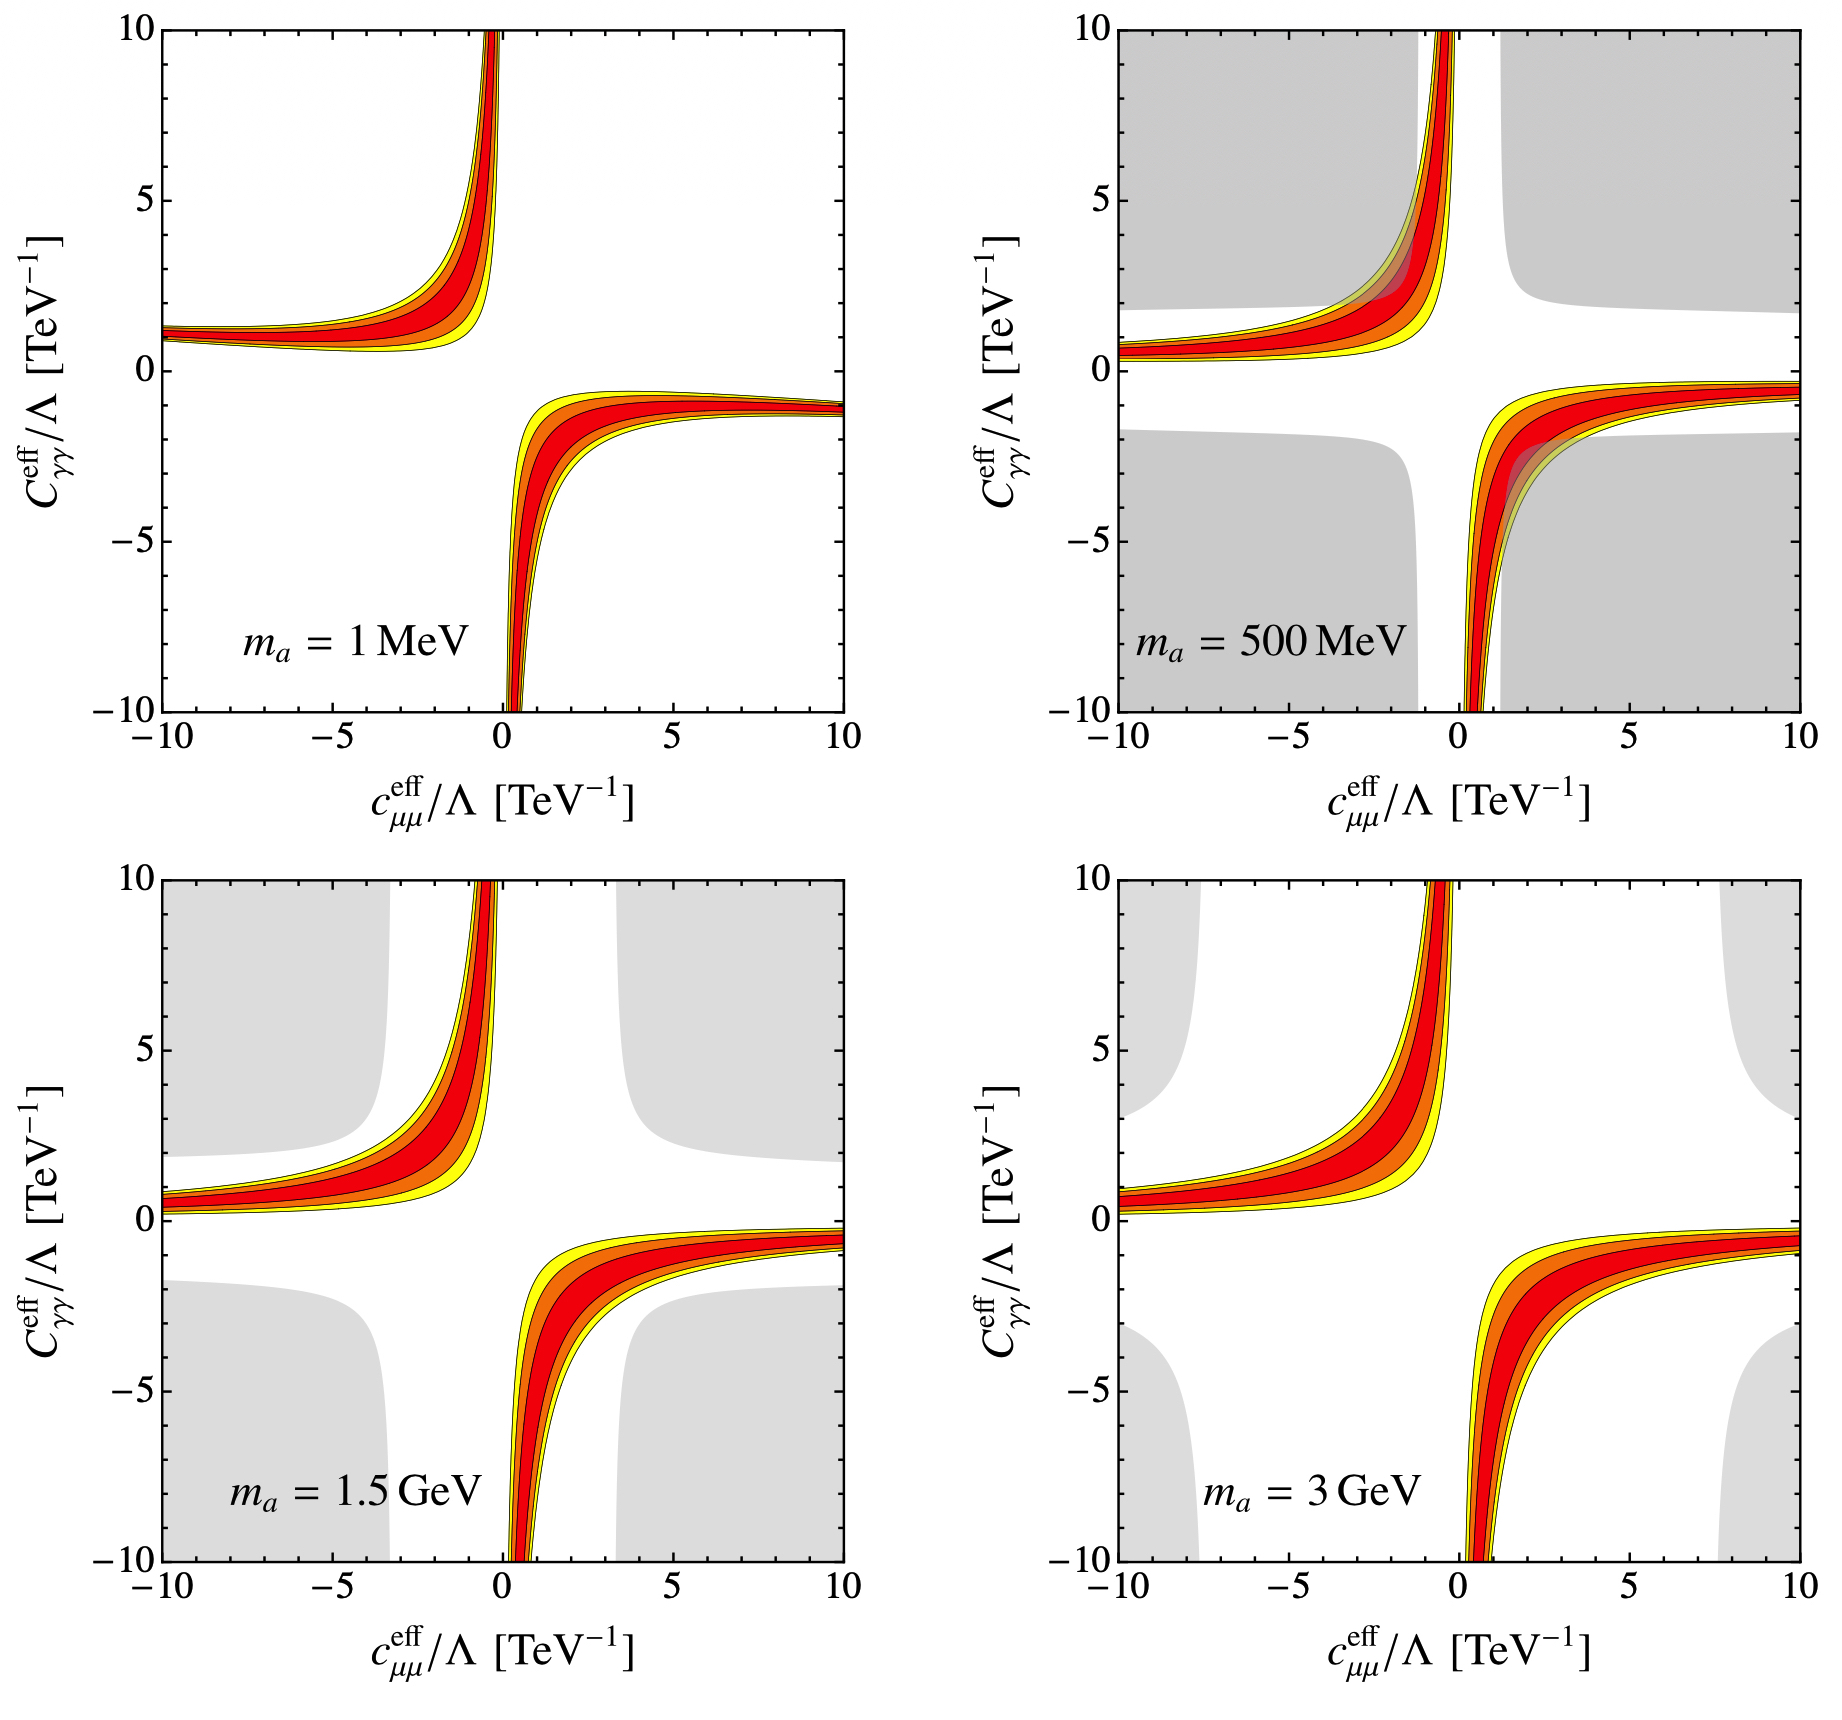
\includegraphics[width=0.85\textwidth]{figures/chapter01/ALP_cuu.jpg}
    \bicaption{\quad \centering 对于不同质量的类轴子,可以在68\%(红色), 95\% (橙色)和99\%(黄色)的置信度上重现$(g-2)_\mu$试验结果的类轴子耦合参数空间。灰色区域表示可以被BaBar实验中对暗光子的寻找所排除的参数空间范围~\cite{Bauer:2017ris}}{\quad \centering Regions in ALP coupling space where the experimental value of $(g-2)_\mu$ is reproduced at 68\% (red), 95\% (orange) and 99\% (yellow) confidence level (CL), for different values of $m_a$. The gray regions are excluded by a dark-photon search performed by BaBar~\cite{Bauer:2017ris}}
    \centering
    \label{fig:c01f03}
\end{figure}

\subsection{冷暗物质候选者}

当类轴子的质量非常小或者与标准模型的相互作用非常弱的时候,类轴子会具有非常长的寿命,这就使得类轴子在衰变到可以被探测器接收到的末态粒子之前就已经飞出了探测器,在探测器中表现为丢失的能量。在这种情况下,类轴子可以作为冷暗物质的候选体~\cite{PhysRevLett.119.031802}。

\subsection{现有研究成果}

图~\ref{fig:c01f04}展示了不同实验对类轴子和光子之间的耦合强度以及类轴子质量的限制范围,横坐标为类轴子的质量,纵坐标为类轴子和光子的耦合强度。其中,红色区域表示可以通过类轴子模型解释实验上观测到的缪子反常磁矩的参数空间范围;淡绿色区域表示在LHC上利用全部二期运行数据对$H\rightarrow Za$衰变道的寻找预计可以排除的类轴子参数空间范围,点线、虚线和实线分别对应于不同的$H\rightarrow Za$耦合强度。因此,大型强子对撞机对类轴子的寻找具有非常高的灵敏度,它可以探测到其他实验所无法探测到的参数空间。此外,通过对$H\rightarrow Za$衰变道的寻找可以让我们对缪子反常磁矩具有更深刻的认识。

\begin{figure}[!htbp]
    \centering
    %trim option's parameter order: left bottom right top
    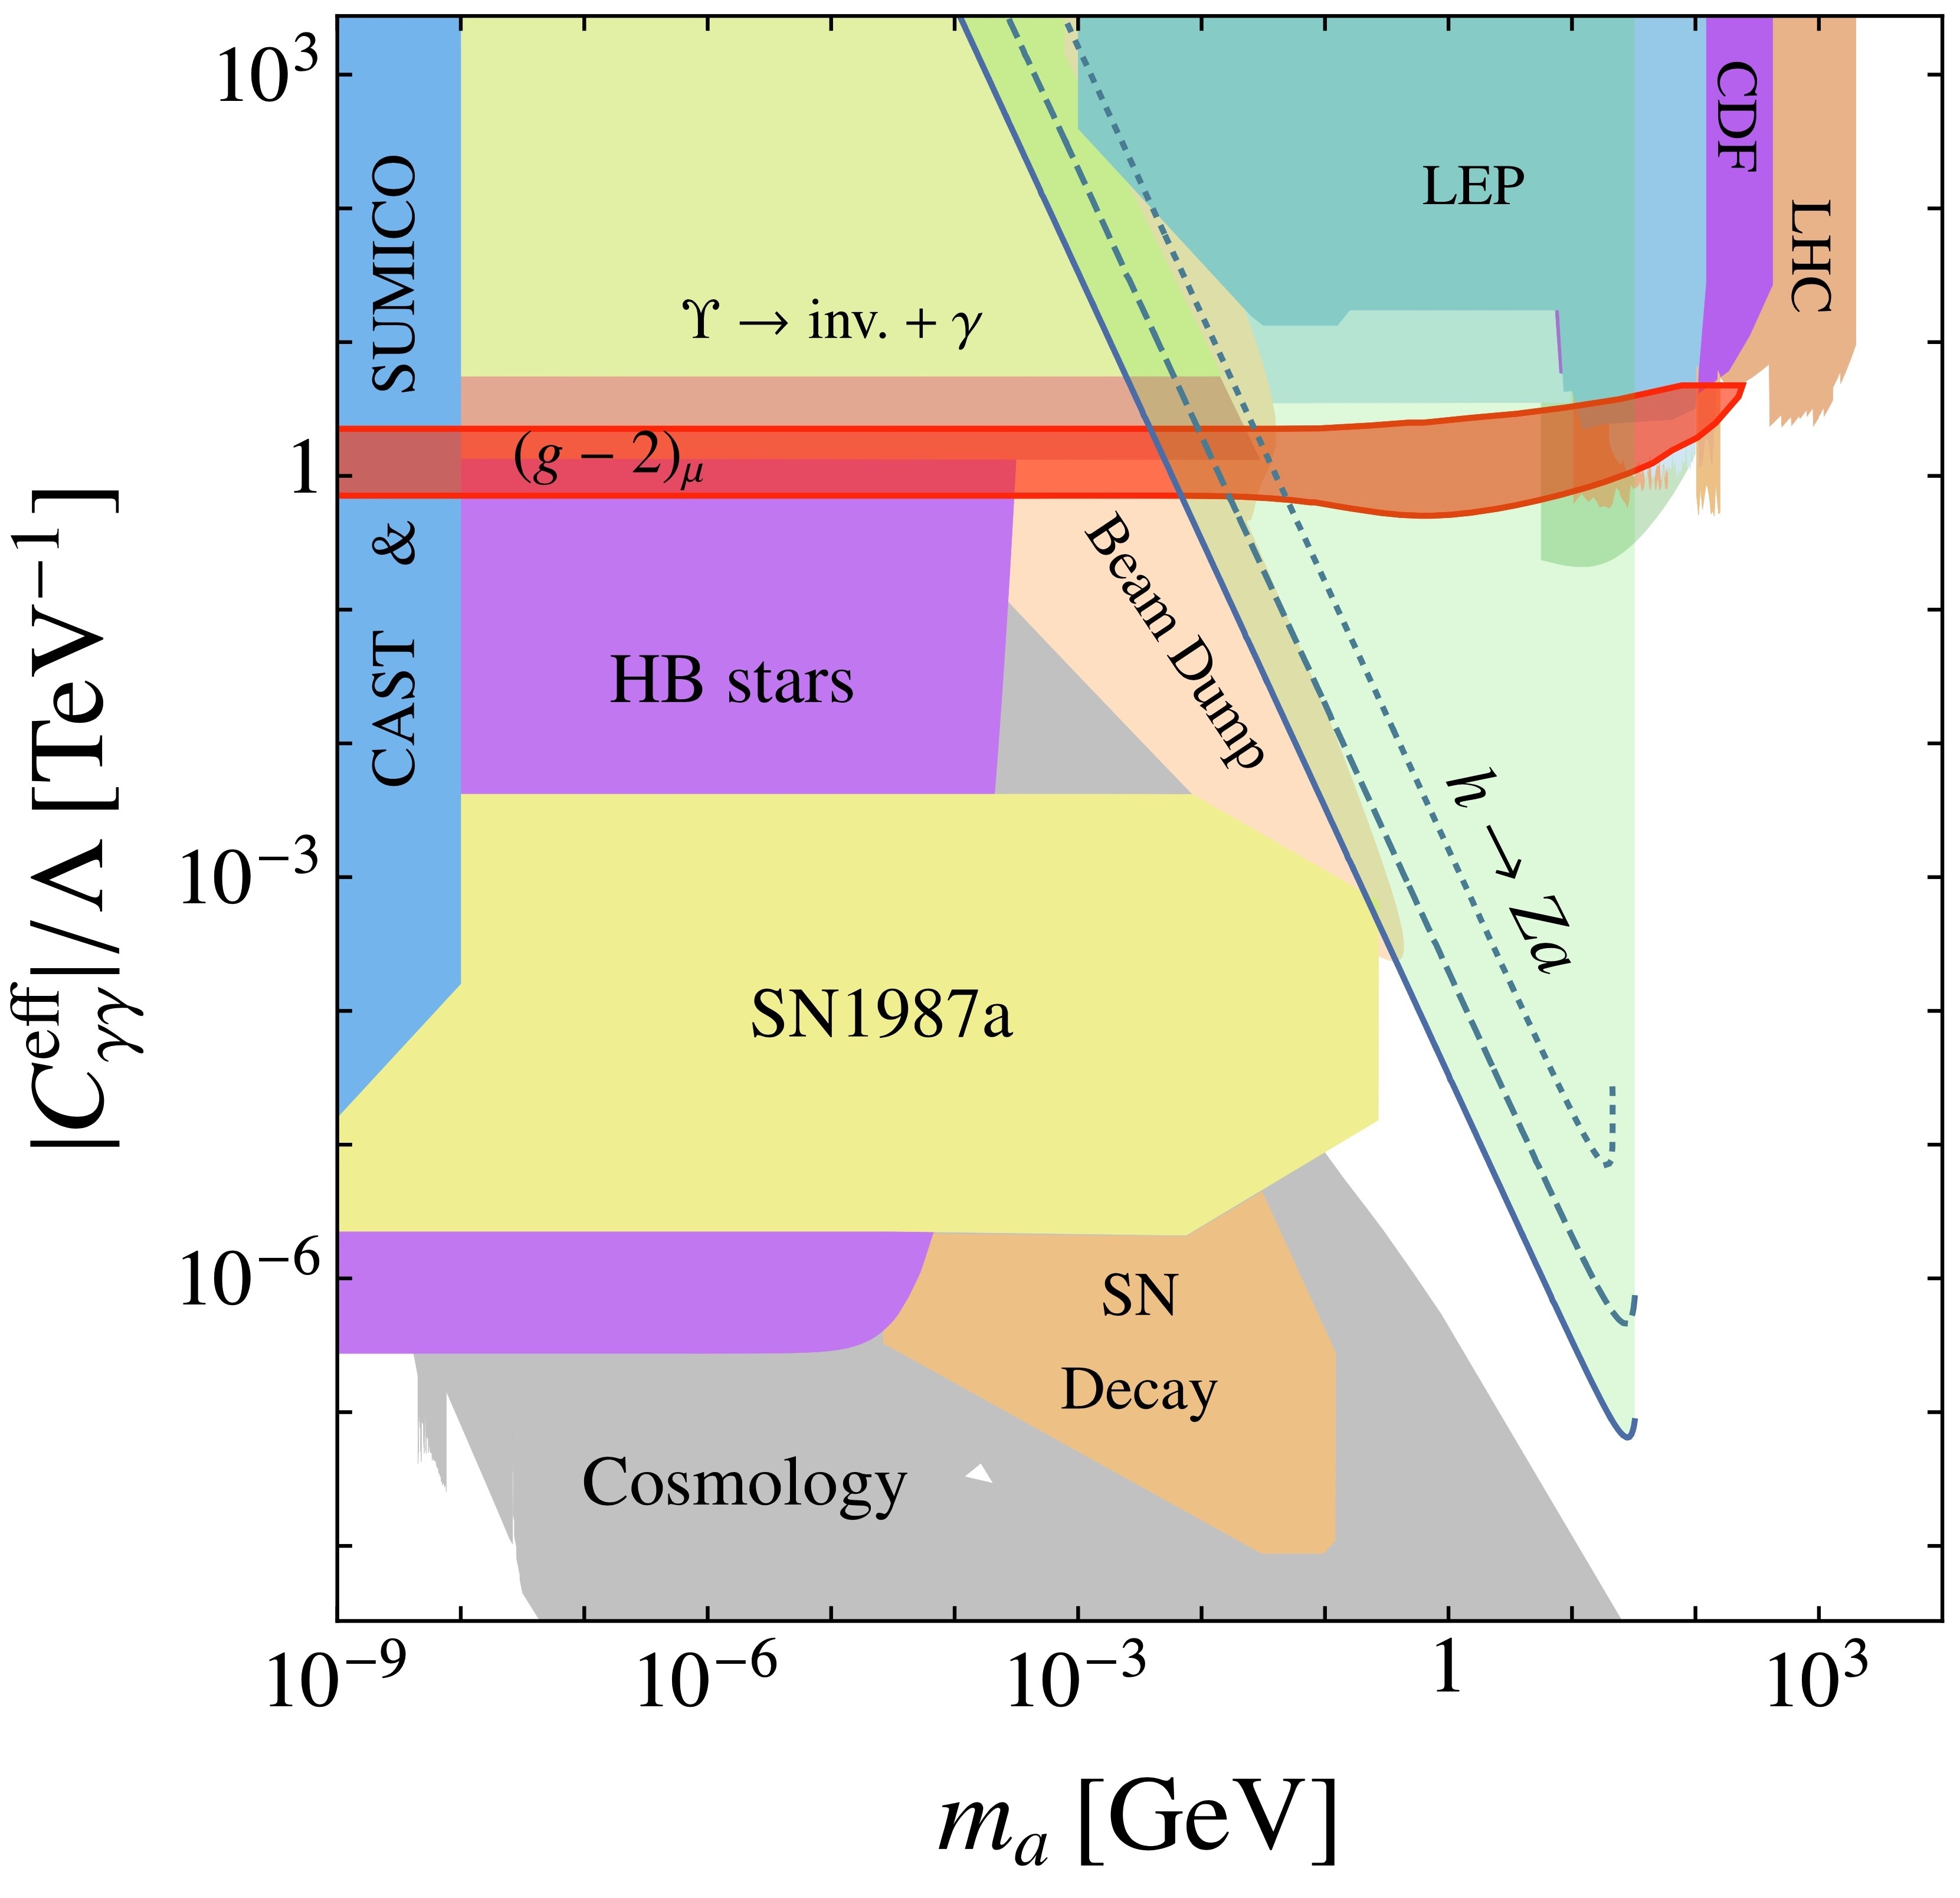
\includegraphics[width=0.70\textwidth]{figures/chapter01/ALP_run2.jpg}
    \bicaption{\quad \centering 不同实验对类轴子质量和与光子之间耦合强度的限制以及可以通过LHC上的$\HZa$衰变道探测的参数空间范围。绿色的点线、虚线和实线轮廓分别对应于$\cZh = 0.72~\si{\TeV^{-1}}$、$0.1~\si{\TeV^{-1}}$、和$0.015~\si{\TeV^{-1}}$。红色区域显示了可以在95\%置信度水平上解释缪子反常磁矩的参数空间~\cite{Bauer:2017ris}}{\quad \centering Constraints on the ALP mass and coupling to photons derived from various experiments along with the parameter regions that can be probed using the Higgs decays $\HZa$ on LHC. The green contours correspond to $\cZh = 0.72~\si{\TeV^{-1}}$ (solid), $0.1~\si{\TeV^{-1}}$ (dashed) and $0.015~\si{\TeV^{-1}}$
    (dotted). The red band shows the preferred parameter space where the $(g-2)_\mu$ anomaly can be explained at 95\% CL~\cite{Bauer:2017ris}}
    \label{fig:c01f04}
\end{figure}

到目前为止,CMS实验和ATLAS实验对不同产生模式和衰变模式下的类轴子进行了寻找。比如:利用Pb--Pb对撞的光子光子散射来寻找类轴子~\cite{aad2021measurement,sirunyan2019evidence};通过研究两个光子在探测器中融合为一个光子喷注来寻找类轴子~\cite{cms2022search,atlas2022search};通过希格斯粒子衰变到四个光子末态来寻找类轴子~\cite{CMS_ALP_1};通过希格斯粒子衰变到四个轻子末态来寻找类轴子~\cite{CMS_ALP_3}。

但是,目前还没有实验对$\HZa$进行过测量。本分析给出了LHC上对希格斯粒子衰变到双轻子加双光子末态的首次测量结果,并且也给出了对类轴子耦合强度的测量结果。

\section{利用希格斯粒子衰变到两轻子加两光子末态来寻找类轴子}

希格斯粒子衰变到一个Z玻色子和一个类轴子的费曼图可以表示为图~\ref{fig:c01f05},其中只考虑了树图水平和单圈图水平。前两项的圈图贡献来自于五维有效拉氏量,最后一项的树图贡献来自于更高阶的有效拉氏量。

\begin{figure}[!htbp]
    \centering
    %trim option's parameter order: left bottom right top
    
\includegraphics[width=0.9\textwidth]{figures/chapter01/ALP_feynman.jpg}
    \bicaption{\quad \centering 对$H\rightarrow Za$有贡献的费曼图~\cite{Bauer:2017ris}}{\quad \centering Feynman diagrams contributing to the decay $H\rightarrow Za$~\cite{Bauer:2017ris}}
    \label{fig:c01f05}
\end{figure}

考虑了所有贡献以后,$H\rightarrow Za$的宽度表达式为
\begin{equation}\label{eq:1-18}
    \Gamma(h \rightarrow Z a)=\frac{m_{h}^{3}}{16 \pi \Lambda^{2}}\left|\frac{C_{\mathrm{Zh}}^{\mathrm{eff}}}{\Lambda}\right|^{2} \lambda^{3 / 2}\left(\frac{m_{Z}^{2}}{m_{h}^{2}}, \frac{m_{a}^{2}}{m_{h}^{2}}\right)
\end{equation}
其中,$\lambda(x,y) = (1-x-y)^2 -4xy$。

在本分析中,Z玻色子最终衰变为两个味道相同、带相反电荷的轻子(电子或缪子);类轴子最终衰变为两个光子,对应的衰变宽度可以表示为
\begin{equation}\label{eq:1-19}
    \Gamma(a \rightarrow \gamma \gamma) \equiv \frac{4 \pi \alpha^{2} m_{a}^{3}}{\Lambda^{2}}\left|C_{\gamma \gamma}^{\mathrm{eff}}\right|^{2}
\end{equation}
对于质量小于两个电子质量的低质量类轴子,标准模型衰变模式中唯一允许的衰变末态是双光子末态。此时,类轴子衰变到双光子会具有非常长的寿命,而且质量越小寿命越长。最终,类轴子会在衰变为可以被探测器捕捉到的两个光子末态之前就飞出探测器,表现为丢失的能量。在此分析中,我们仅关注希格斯粒子的奇异衰变,因此类轴子衰变到双光子末态的分支比被设定为100\%。

根据$H\rightarrow Za$的动力学性质,由于我们要求一个在壳的Z玻色子,由希格斯粒子衰变而来的低质量类轴子会具有非常高的横动量,使得类轴子衰变产生的两个光子具有非常小的角距离,最终在探测器里会表现为一个融合的光子喷注。此时,$H\rightarrow Za$会对$H\rightarrow Z\gamma$的宽度测量产生贡献,使得$H\rightarrow Z\gamma$的宽度测量相对于标准模型的预言偏大。图~\ref{fig:c01f06}展示了$h \rightarrow Z a$的宽度和标准模型$h \rightarrow Z \gamma$宽度的比值作为有效威尔逊系数$\cZh$的函数,在一定参数空间,类轴子可以对标准模型$h \rightarrow Z \gamma$的寻找产生很大的影响。

\begin{figure}[!htbp]
    \centering
    %trim option's parameter order: left bottom right top
    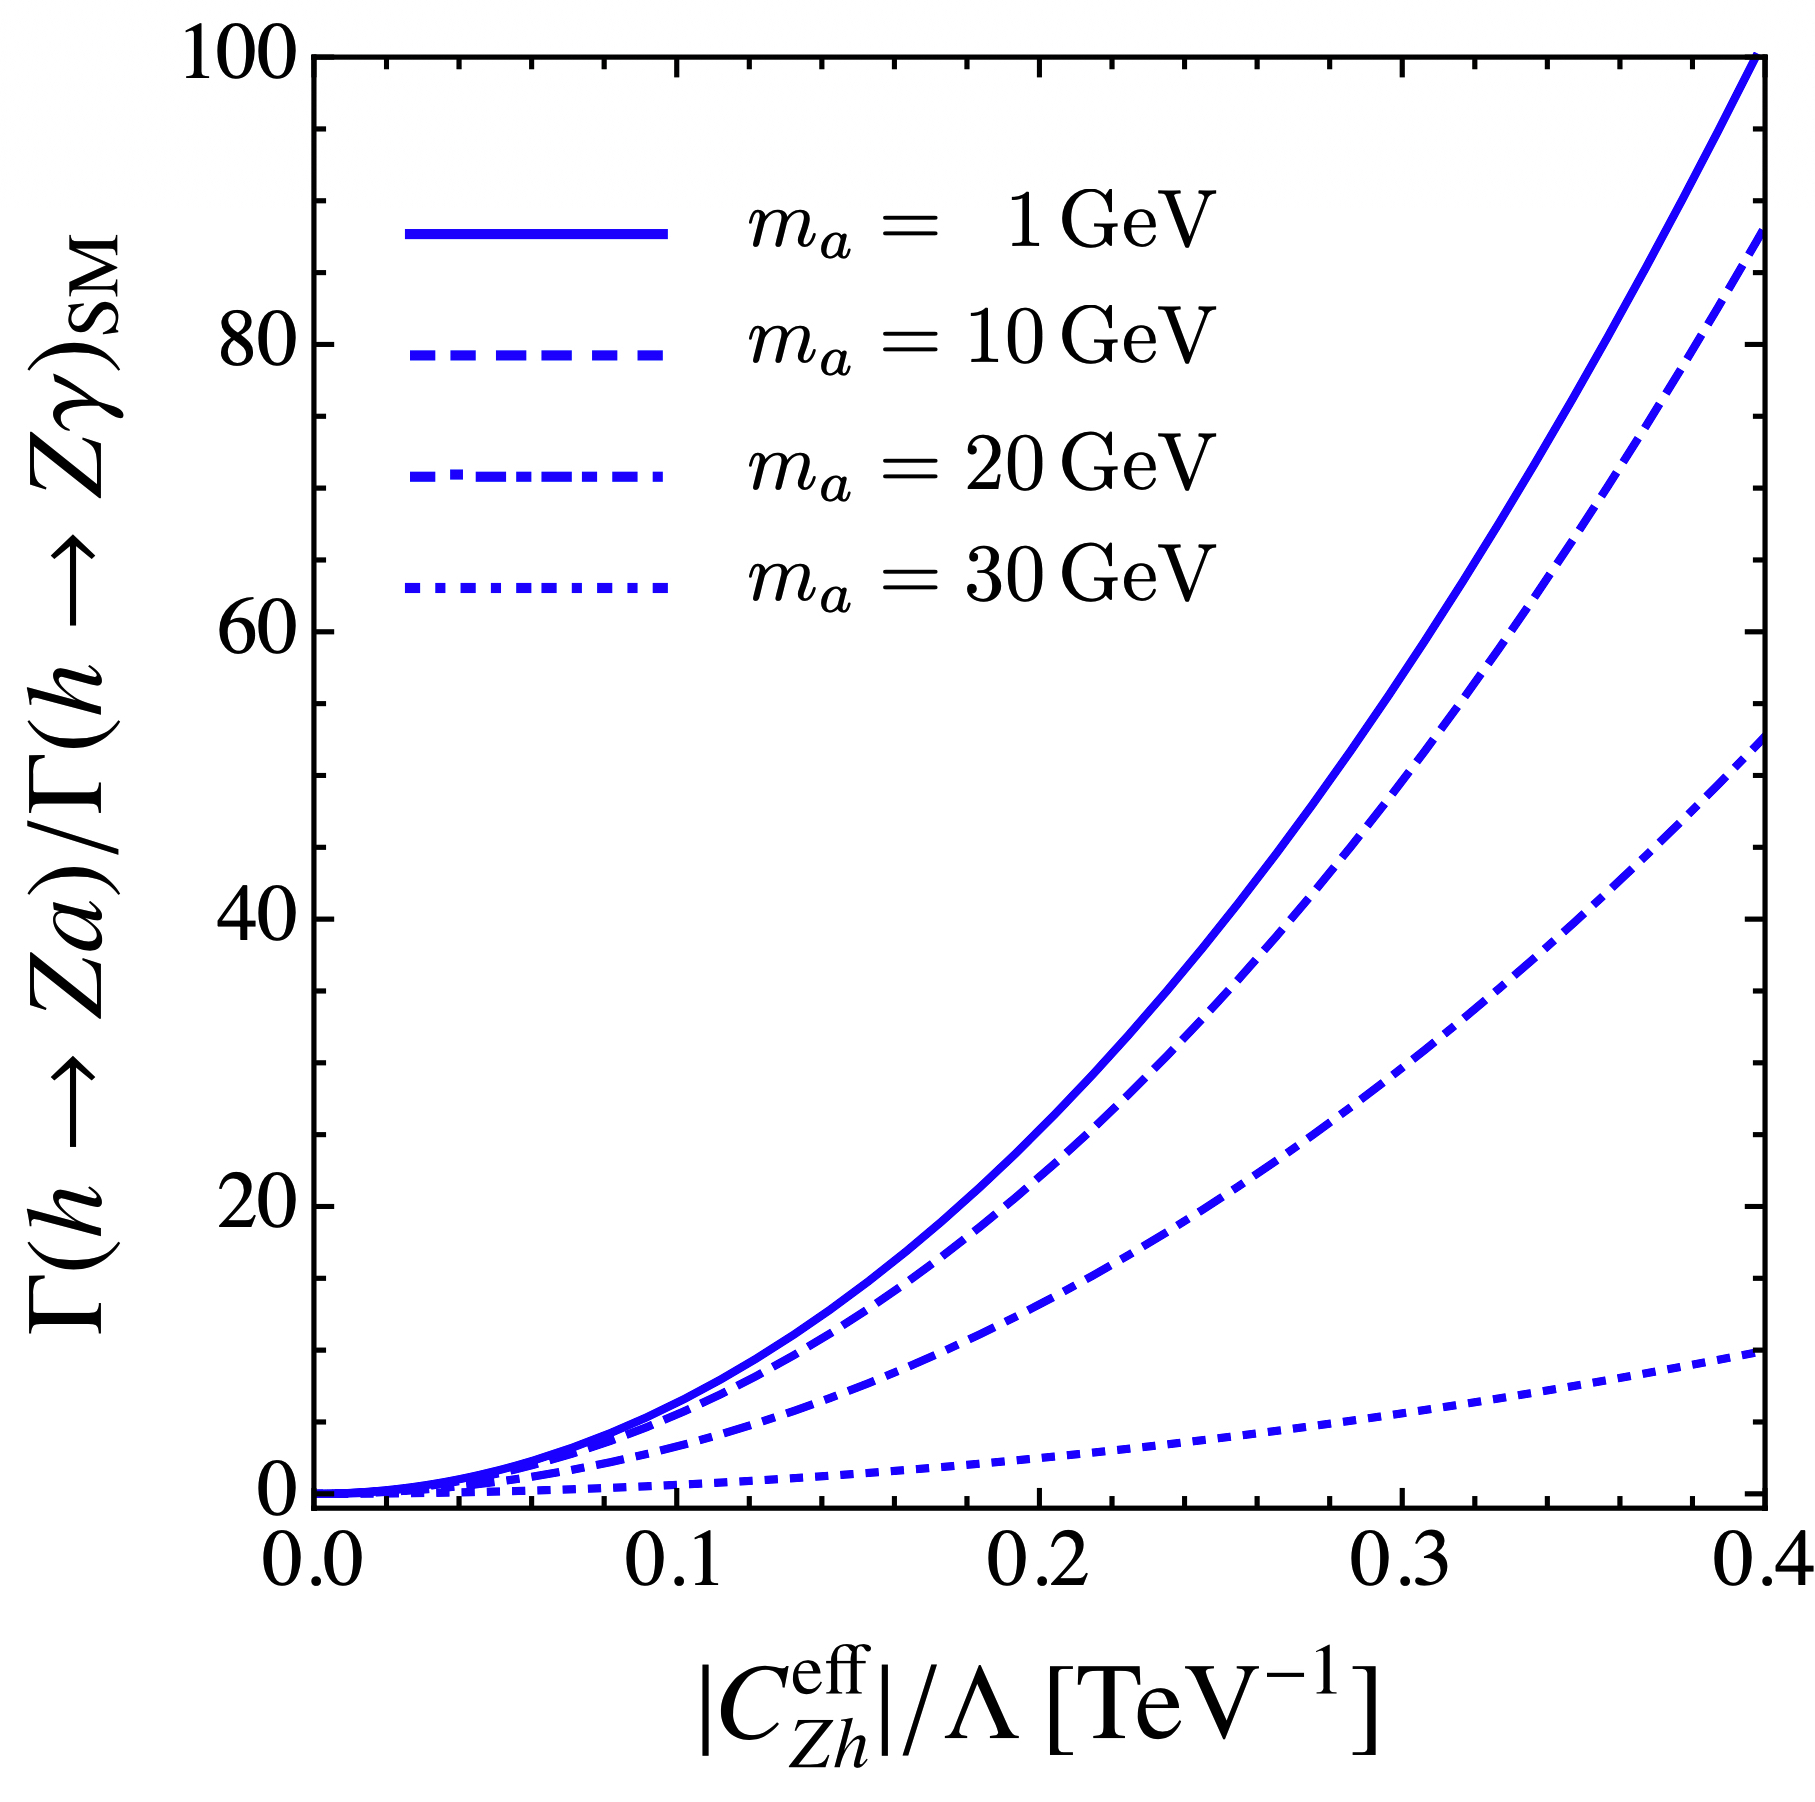
\includegraphics[width=0.5\textwidth]{figures/chapter01/ALP_GammaRatio.jpg}
    \bicaption{\quad \centering 对于不同的类轴子质量,比值$\Gamma(h \rightarrow Z a) / \Gamma(h \rightarrow Z \gamma)_{\mathrm{SM}}$作为有效威尔逊系数$\cZh$的函数~\cite{Bauer:2017ris}}{\quad \centering The ratio of $\Gamma(h \rightarrow Z a) / \Gamma(h \rightarrow Z \gamma)_{\mathrm{SM}}$ as a function of the effective Wilson coefficient $\cZh$ for different ALP masses~\cite{Bauer:2017ris}}
    \label{fig:c01f06}
\end{figure}

\subsection{研究的物理意义}

首先,此研究可以作为与模型无关的低质量双光子共振态的寻找。到目前为止,LHC上尚未有希格斯粒子衰变到双光子加双轻子末态的测量结果,此分析给出了希格斯粒子在双轻子加双光子末态下的首次测量结果,并对质量范围为1--30$\GeV$之间的低质量双光子共振态进行了寻找,让我们对希格斯粒子的奇异衰变有了更深刻的理解。

其次,此分析首次利用了$\HZa$衰变道对类轴子进行了寻找。根据图~\ref{fig:c01f04}所示,在LHC上通过$\HZa$衰变道对类轴子的寻找具有非常高的灵敏度,测量结果可以覆盖到其他实验所不能探测的参数空间。此外,在一定的参数空间范围中,类轴子模型可以解释实验上观测到的缪子反常磁矩的物理现象,对类轴子的寻找可以让我们对缪子反常磁矩具有更深刻的理解。

\subsection{研究难点}

首先,本分析所要求的信号事例末态两个光子的横动量比较低。由于要求Higgs衰变产生一个在壳的Z玻色子和类轴子,根据衰变的动力学分析,类轴子的质量大概在小于30$\GeV$的范围内。因此,信号事例末态两个光子的横动量大部分集中在10$\GeV$到15$\GeV$之间。而在CMS实验中,默认的光子辨别算法要求横动量大于15$\GeV$,这就使得传统默认的CMS光子辨别算法不再适用于本分析。

其次,在低质量类轴子区间(小于5$\GeV$),信号事例末态两个光子的角距离非常小。由于类轴子的质量非常小,使得从希格斯粒子衰变产生的类轴子具有比较高的横动量,进而使得类轴子衰变产生的两个光子具有非常高的横动量,使得这两个光子具有非常小的角距离,无法在探测器中识别并重建出两个光子。

最后,本分析具有非常低的信噪比。由于在信号区间存在大量的假光子和与信号事例无关的标准模型过程等本底,使得最终的信号显著度非常低。

\subsection{研究方法}

本分析利用了CMS探测器整个二期运行期间(2016年、2017年和2018年)收集到的138~\si{fb^{-1}}的数据对$\HZa$进行了寻找,其中轻子部分仅包括电子和缪子。针对以上难点,本分析提供了以下解决办法。

首先,本分析研究了传统光子辨别算法中各个变量对信号事例的影响,设计了新的光子鉴别算法,使得信号效率在低质量区间获得了显著的提升。

为了进一步提高信号显著度,本分析采用了多变量分析的方法,利用光子和类轴子的动力学等信息作为输入对信号和本底进行区分,最终使得信号显著度获得了显著的提升。
